\documentclass[11pt,aspectratio=169]{beamer}
\usepackage[utf8]{inputenc}
\usepackage[T1]{fontenc}
\usepackage{graphicx}
\usetheme{default}
\usecolortheme{beaver}
\usepackage{url}
\usepackage[export]{adjustbox}
\usepackage{pdfpcnotes}

\begin{document}
	\author{Niklas Fuhrberg, Anton Schirg,\\ Christian Schwarz, Janis Streib, Bob Weinand}
	\title{MAMID}
	\subtitle{Monitor and Manager for In-Memory Databases\\Functional Specification}
	%\logo{}
	\institute{\textbf{Supervisor}\\Dr. Marek Szuba\\SCC}
	\date{8 June 2016}
	\subject{Functional Specification}
	%\setbeamercovered{transparent}
	%\setbeamertemplate{navigation symbols}{}
	\frame[plain]{\maketitle}
	
	\begin{frame}{Requirements Elicitation}
		\pnote{Start with requirements elicitation phase.}
		\pnote{Requirements derived from interview with Marek and Administrator}
		MongoDB Database Cluster \pnote{We knew from the beginning: Manager for MongoDB}
		\begin{itemize}
			\item<2-> Replica Sets 	\pnote{specifically, management of replica sets}
			\item<3-> low maintenance effort \pnote{little time for maintaining the cluster hosts \& MongoDB deployment}
			\item<4-> volatile storage \pnote{volatility of the host storage is the core problem (hence the title of the project)}
			\item<5-> physical interdependencies \pnote{machines are organized in cabinets sharing power supply -> pick replica set members carefully}
			\item<6-> automation \pnote{the admin does not want to reconfigure instances after every reboot}
			\item<7-> monitoring \pnote{high-availibility of data is required by consumers of MongoDB deployment}
		\end{itemize}
	\end{frame}
	
	
	\begin{frame}{Requirements Analysis}
		\pnote{not configure, only desc functionality + constraints of the cluster}
		\pnote{saves time} \pnote{setup is self-describing: mamid web interface is all a new admin needs to get started / existent admin does not remember config from 2 years ago\\}
		
		\pnote{the description of the cluster => set of constraints to the deployment}
		\pnote{RISK GROUPS (model shared risk)}
		\pnote{PERSISTENCE OF HOST STORAGE (models exactly this, req to guarantee persistence in case of power loss)}
		\pnote{MEMBER COUNTS (model degree of redundancy \& performance gain through horizontal scaling)\\}

		\pnote{after layout is determined, we need to actually run it}
		\pnote{here, mamid = simple configuration engine}
		\pnote{takes description of desired state of a host and deploys it using daemons on all cluster hosts}
		\pnote{deploy = spawn mongods, configure replica sets, etc\\}

		\pnote{once deployed, need to check whether just deployed layout is actually the one that's running}
		\pnote{concisely = check for divergence between ideal layout and the reality}
		\pnote{monitor that\\
			continously monitors mongods and their configuration\\
			notifies administrator about problems in the cluster\\
			triggers automatic redeployment if divergence detected\\
			=> SPECIFICALLY covers the case of a volatile host going down (come to that in a sec)\\}

		\pnote{no manual config of mongod through administrator, done by mamid}
		\pnote{only MongoDB. Parts are fairly generic, parts are specific. Design can account for this but given what we learned in the interview, other DBs are not the primary goal of the project.}
		\pnote{sharding only in so far that we provide config-sever compatible configuration profile}

		\begin{columns}
			\begin{column}{0.5\linewidth}
				Features
				\pause
				\begin{itemize}
					\item<2-> declarative approach
					\item<3-> automatic cluster layout
					\item<4-> automatic deployment
					\item<5-> continuous monitoring
				\end{itemize}
			\end{column}
			\begin{column}{0.5\linewidth}
				\onslide<6->{Demarcation}
				\begin{itemize}
					\item<7-> no manual configuration
					\item<8-> only MongoDB
					\item<9-> no query router deployment
				\end{itemize}
				\vspace{1.5em} % dirty hacks
			\end{column}
		\end{columns}

	\end{frame}
	
	\begin{frame}<4>[label=screenshots]
		\frametitle{Walkthrough} \pnote{Make you familiar with the terminology and a basic cluster setup process}
		\begin{center}
			\only<1>{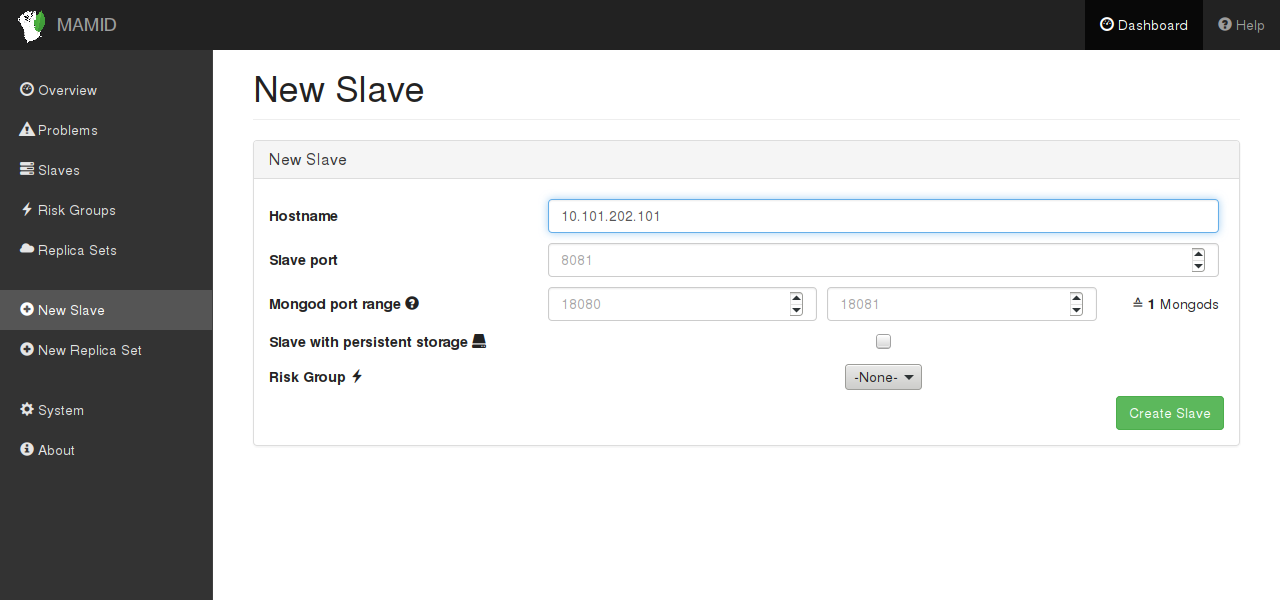
\includegraphics[height=0.8\textheight,frame]{screenshots/new_slave}}
			\only<2>{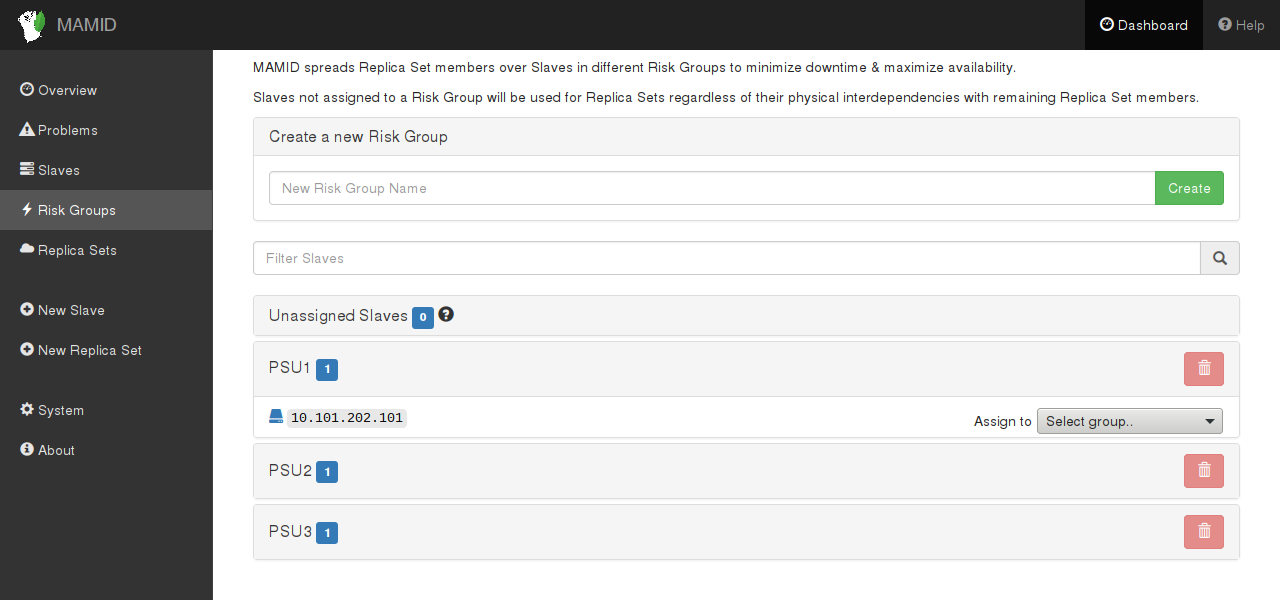
\includegraphics[height=0.8\textheight,frame]{screenshots/risk_groups}}
			\only<3>{\includegraphics[height=0.8\textheight,frame]{screenshots/new_replica_set}}
		\end{center}
	\end{frame}
	
	\begin{frame}<8>[label=hwlayout]
		\frametitle{Walkthrough}
			\only<1>{
\includegraphics[width=0.9\linewidth]{assets/cluster_hw_stepwise/step1}}
			\only<2>{
\includegraphics[width=0.9\linewidth]{assets/cluster_hw_stepwise/step2}}
			\only<3>{
\includegraphics[width=0.9\linewidth]{assets/cluster_hw_stepwise/step3}}
			\only<4>{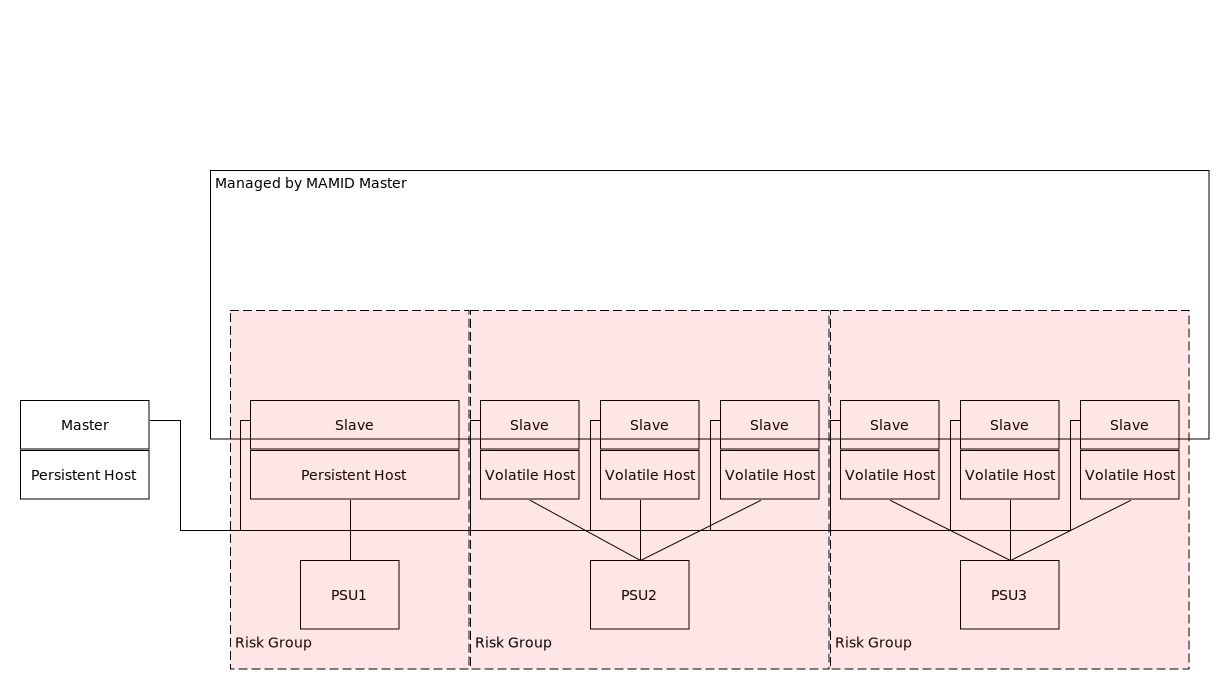
\includegraphics[width=0.9\linewidth]{assets/cluster_hw_stepwise/step4}}
			\only<5>{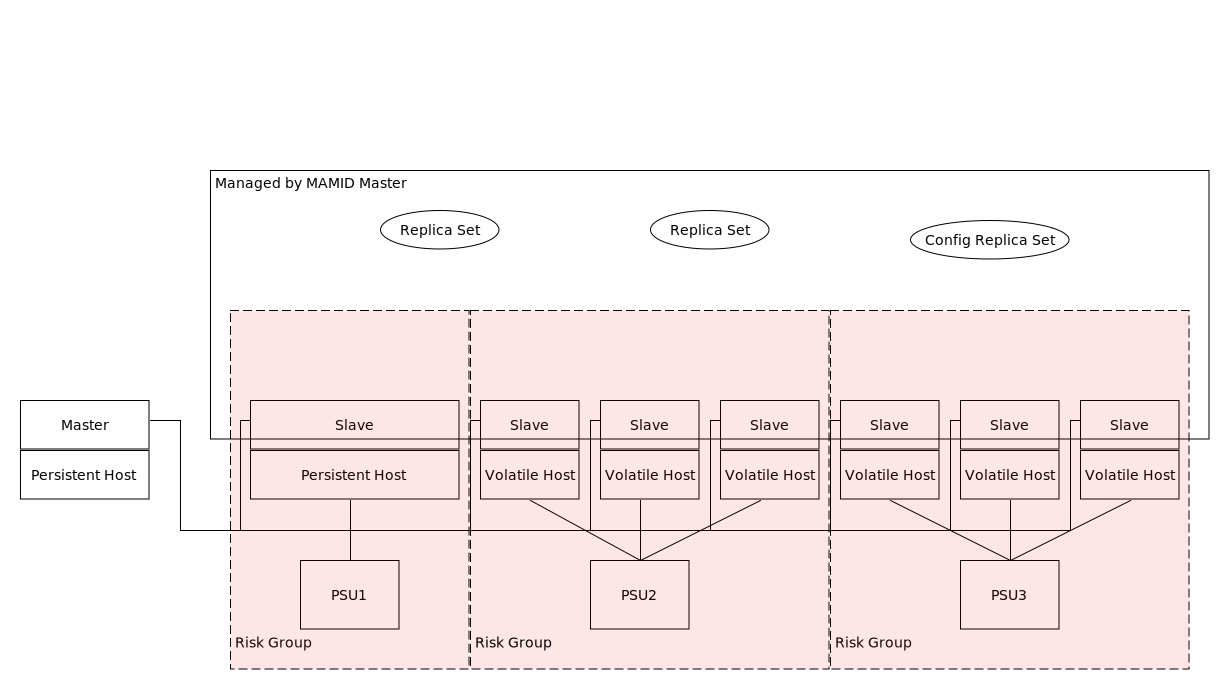
\includegraphics[width=0.9\linewidth]{assets/cluster_hw_stepwise/step5}}
			\only<6>{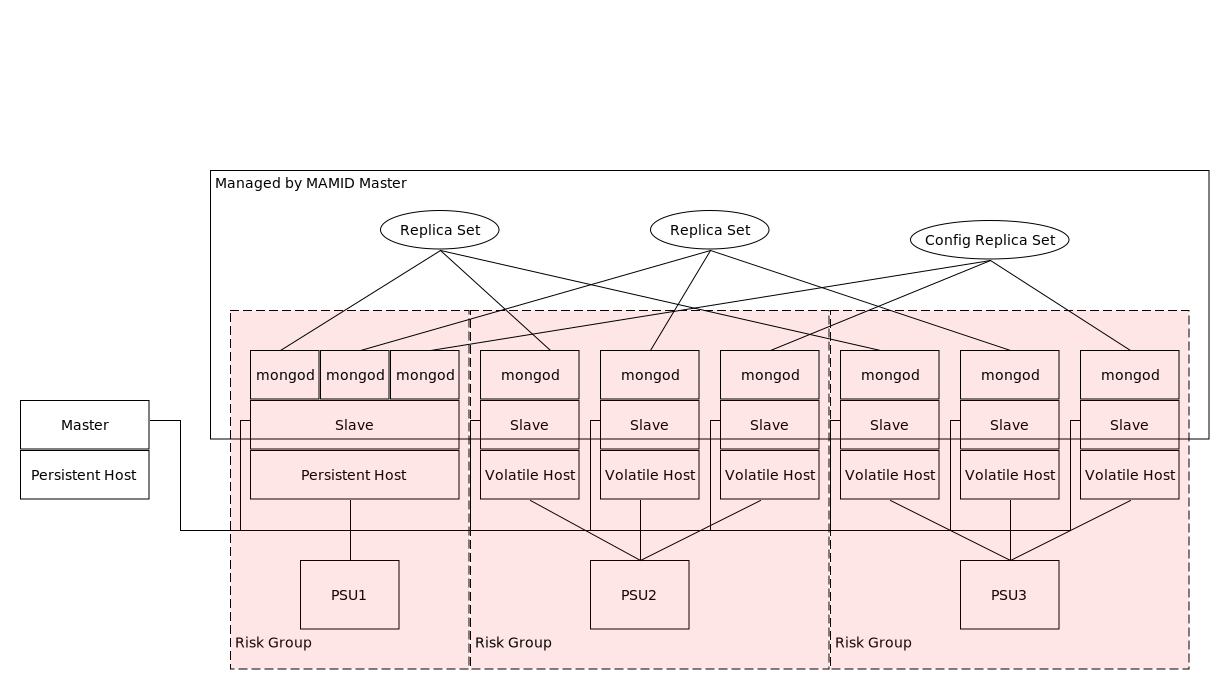
\includegraphics[width=0.9\linewidth]{assets/cluster_hw_stepwise/step6}}
			\only<7>{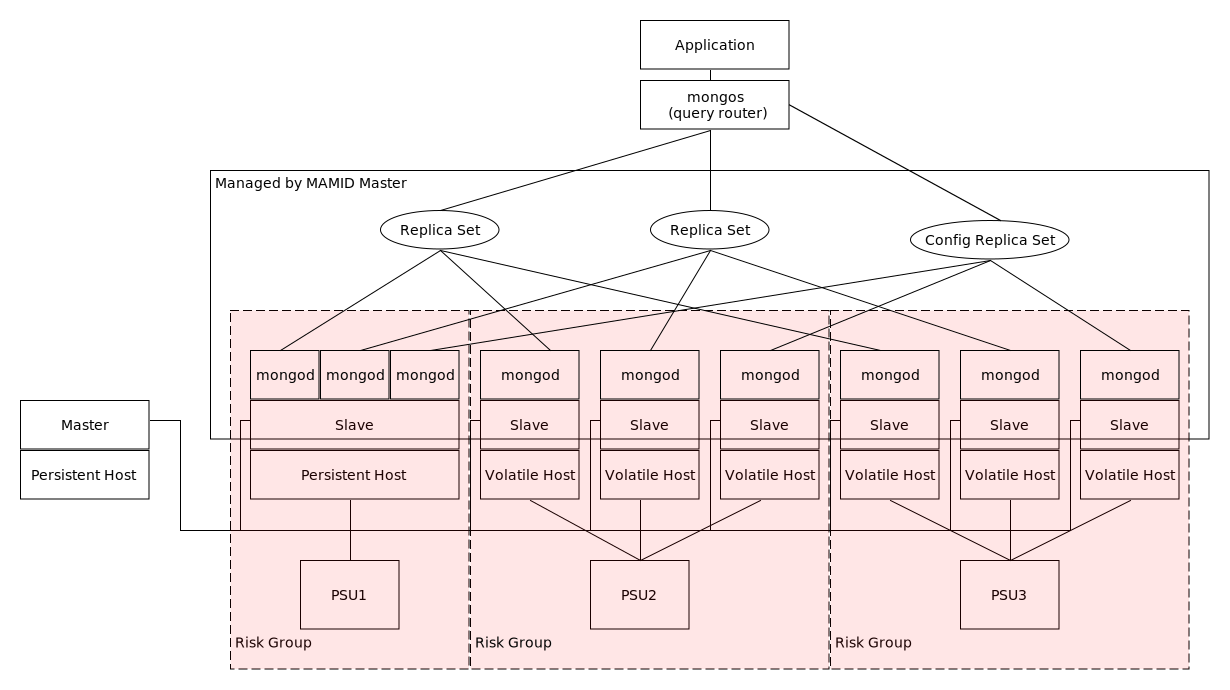
\includegraphics[width=0.9\linewidth]{assets/cluster_hw_stepwise/step7}}
			%dirty hack: repeat to avoid second blank slide
			\only<8>{
\includegraphics[width=0.9\linewidth]{assets/cluster_hw_stepwise/step1}}
	\end{frame}

	\againframe<1>{screenshots}
	\againframe<1>{hwlayout}	
	\againframe<3>{hwlayout}
	\againframe<2>{screenshots}
	\againframe<3>{hwlayout}
	\againframe<4>{hwlayout}
	\againframe<3>{screenshots}
	\againframe<4>{hwlayout}
	\againframe<5>{hwlayout}
	\againframe<6>{hwlayout}
	\againframe<7>{hwlayout}
	
	\begin{frame}<1-13>
		\frametitle{Failure Scenario: Power Supply Outage} \pnote{Now come to the most important scenario: failure + data loss}
		\only<2>{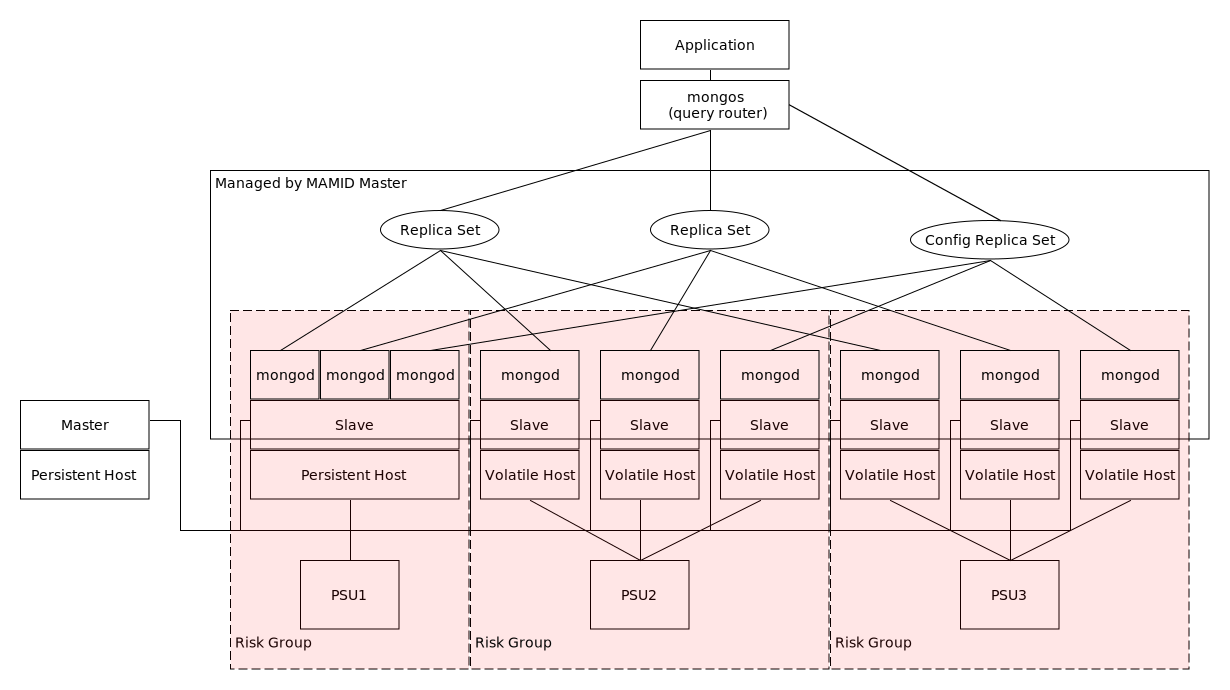
\includegraphics[width=0.9\linewidth]{assets/cluster_hw_stepwise/step7}}
		\only<3>{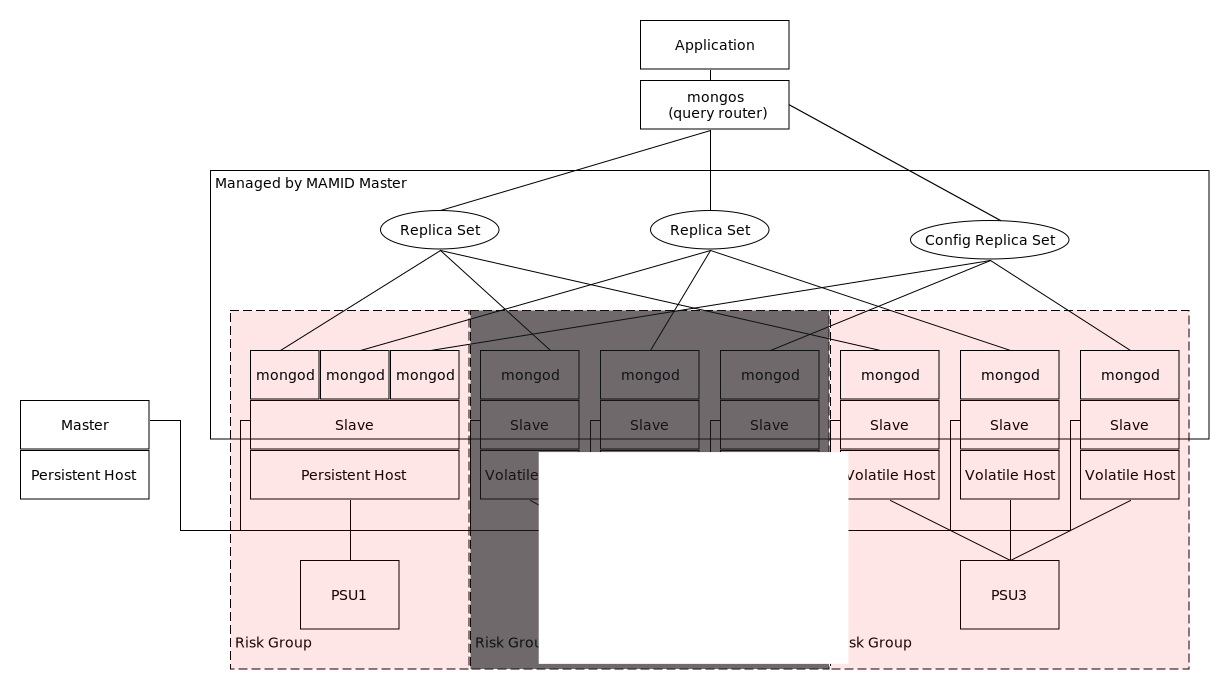
\includegraphics[width=0.9\linewidth]{assets/cluster_hw_stepwise/step8}}
		\only<4>{\centering 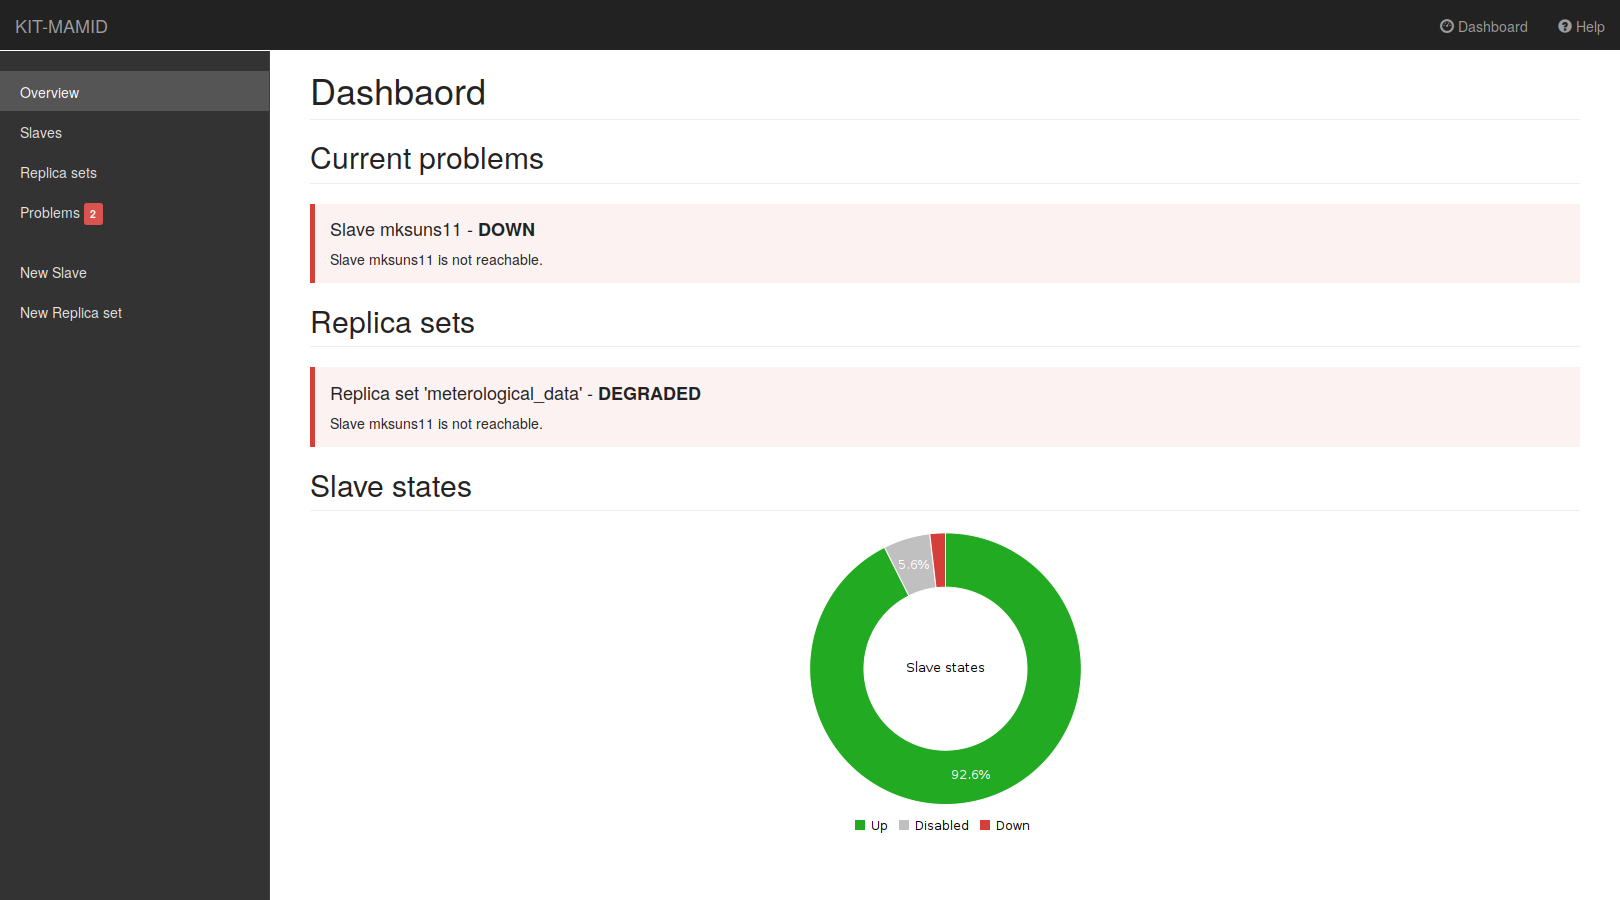
\includegraphics[height=0.8\textheight,frame]{screenshots/dashboard}}
		\only<5>{\centering \includegraphics[height=0.8\textheight,frame]{screenshots/slave_edit_unknown}}
		\only<6>{\centering \includegraphics[height=0.8\textheight,frame]{screenshots/replica_set_overview_degraded}}
		\only<7>{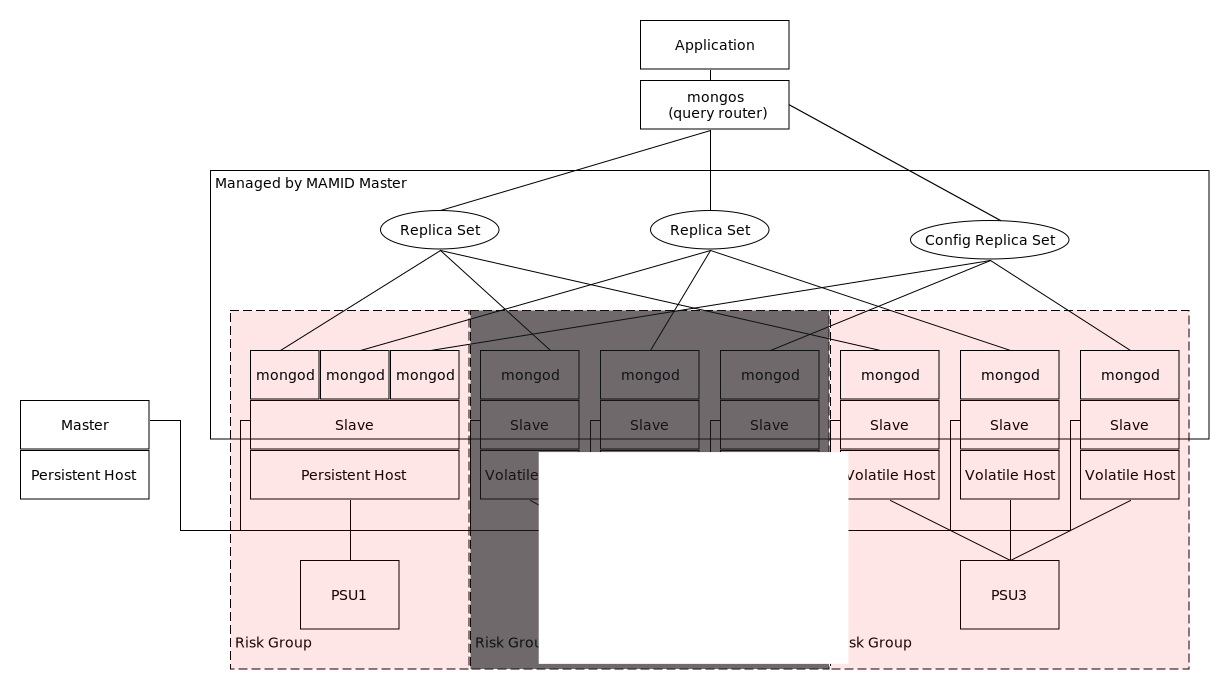
\includegraphics[width=0.9\linewidth]{assets/cluster_hw_stepwise/step8}}
		\only<8>{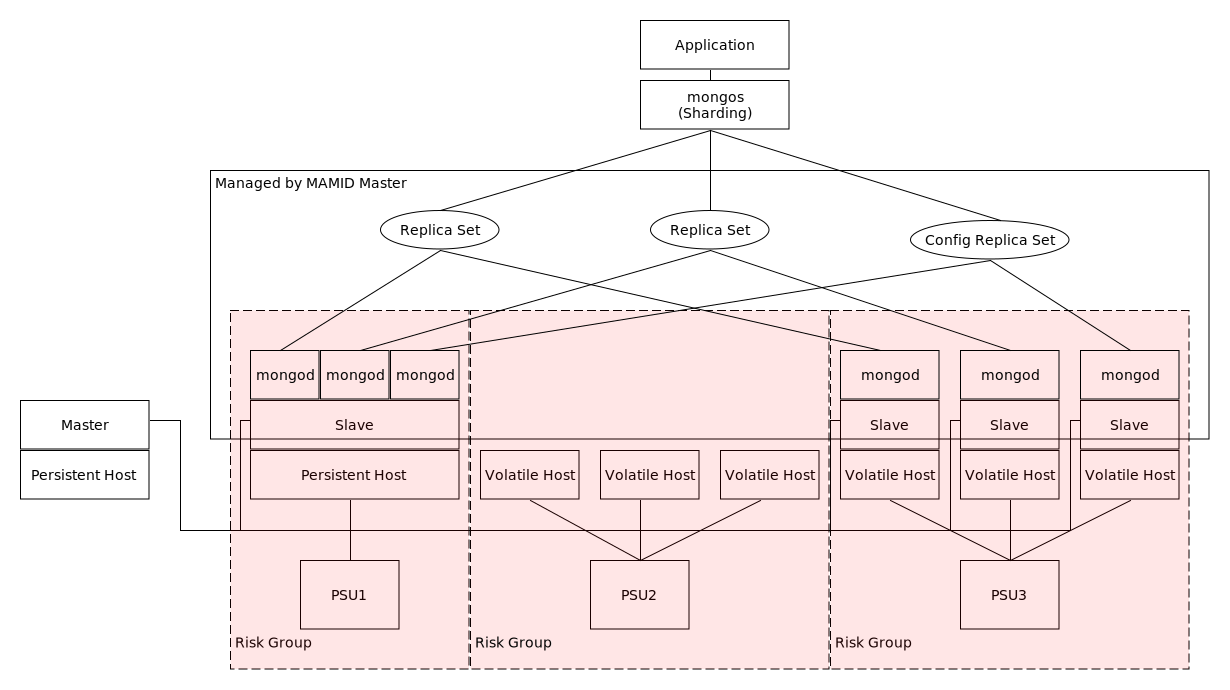
\includegraphics[width=0.9\linewidth]{assets/cluster_hw_stepwise/step9}}
		\only<9>{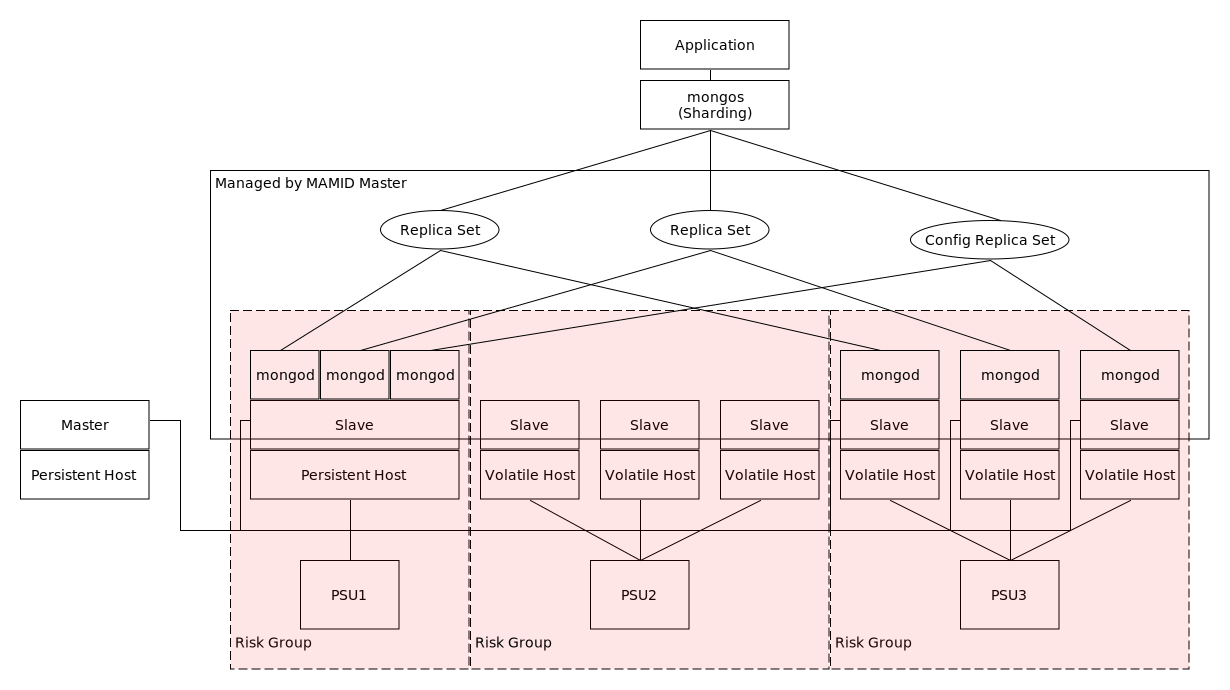
\includegraphics[width=0.9\linewidth]{assets/cluster_hw_stepwise/step10}}
		\only<10>{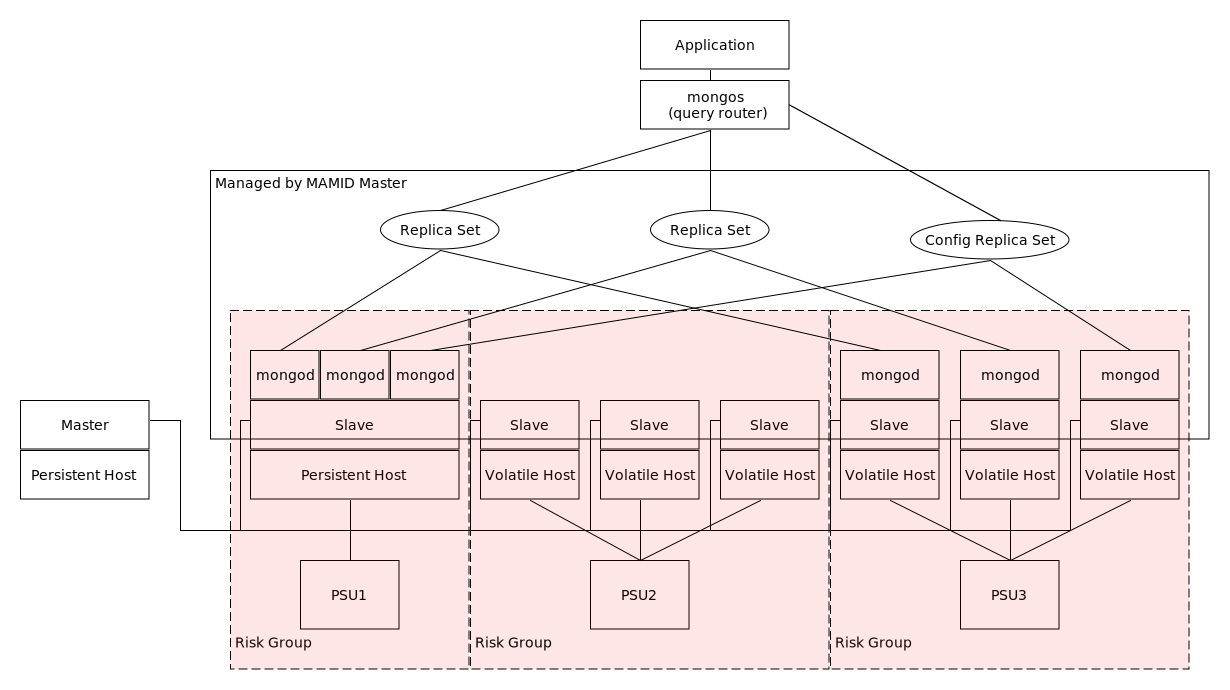
\includegraphics[width=0.9\linewidth]{assets/cluster_hw_stepwise/step11}}
		\only<11>{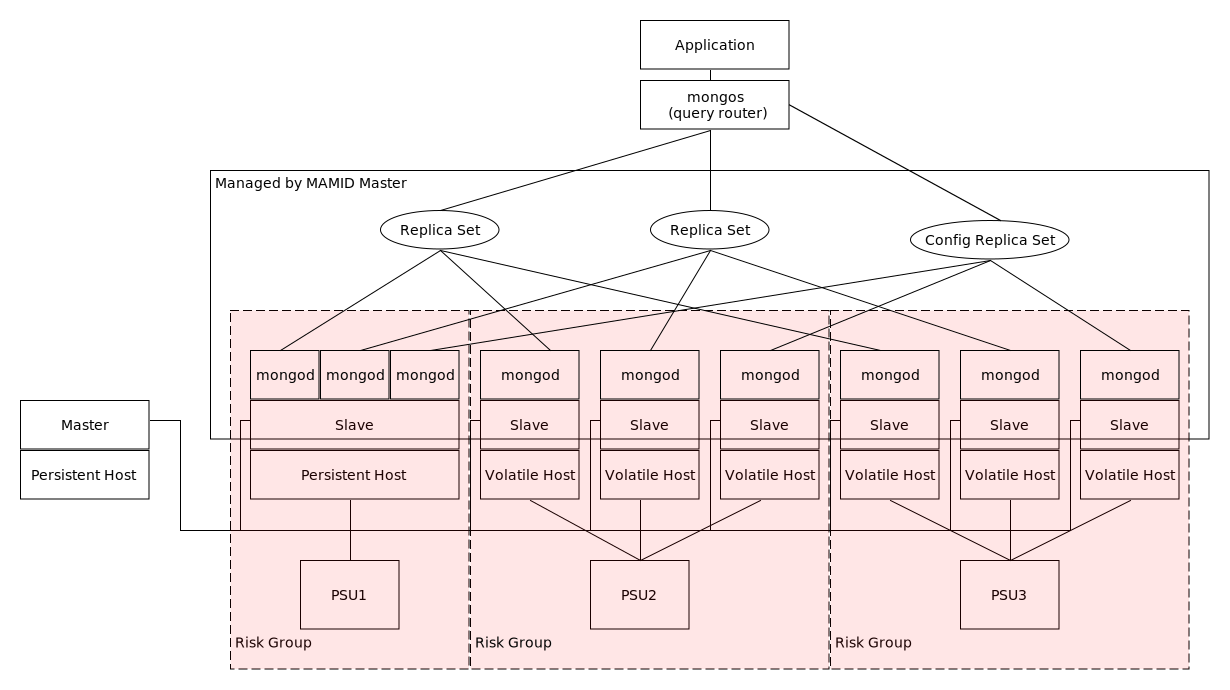
\includegraphics[width=0.9\linewidth]{assets/cluster_hw_stepwise/step7}}
		\only<12>{\centering \includegraphics[height=0.8\textheight,frame]{screenshots/slave_edit_active}}
		\only<13>{\centering \includegraphics[height=0.8\textheight,frame]{screenshots/replica_set_overview_active}}
	\end{frame}
	
	\begin{frame}{Questions?}
		\centering
		\begin{figure}
			\includegraphics[height=0.7\textheight,frame]{assets/xkcd1289}
			\caption{\tiny Randall Munroe | CC BY-NC 2.5 | \url{https://xkcd.com/1289}}
		\end{figure}
		
	\end{frame}
	
\end{document}
